%%%%%%%%%%%%%%%%%%%%%%%%%%%%%%%%%%%%%%%%%%%%%%%%%%%%%%%%%%%%%%%%%%
%%%%%%%% ICML 2014 EXAMPLE LATEX SUBMISSION FILE %%%%%%%%%%%%%%%%%
%%%%%%%%%%%%%%%%%%%%%%%%%%%%%%%%%%%%%%%%%%%%%%%%%%%%%%%%%%%%%%%%%%

% Use the following line _only_ if you're still using LaTeX 2.09.
%\documentstyle[icml2014,epsf,natbib]{article}
% If you rely on Latex2e packages, like most moden people use this:
\documentclass{article}

% use Times
\usepackage{times}
% For figures
\usepackage{graphicx} % more modern
%\usepackage{epsfig} % less modern
\usepackage{subfigure} 

% use formatting for item enumeration
\usepackage{enumitem}

% For citations
\usepackage{natbib}

% For algorithms
\usepackage{algorithm}
\usepackage{algorithmic}

% As of 2011, we use the hyperref package to produce hyperlinks in the
% resulting PDF.  If this breaks your system, please commend out the
% following usepackage line and replace \usepackage{icml2014} with
% \usepackage[nohyperref]{icml2014} above.
\usepackage{hyperref}

% Packages hyperref and algorithmic misbehave sometimes.  We can fix
% this with the following command.
\newcommand{\theHalgorithm}{\arabic{algorithm}}

% Employ the following version of the ``usepackage'' statement for
% submitting the draft version of the paper for review.  This will set
% the note in the first column to ``Under review.  Do not distribute.''
\usepackage{icml2014} 
%\usepackage{multicols}


% The \icmltitle you define below is probably too long as a header.
% Therefore, a short form for the running title is supplied here:
\icmltitlerunning{Kotfis, Li, Ouyang}

\begin{document} 

\twocolumn[
\icmltitle{BroadMind: A Better Platforming Agent}

% It is OKAY to include author information, even for blind
% submissions: the style file will automatically remove it for you
% unless you've provided the [accepted] option to the icml2014
% package.
\icmlauthor{Dave Kotfis}{dkotfis@seas.upenn.edu}
\icmlauthor{Zhi Li}{zhili@seas.upenn.edu}
\icmlauthor{Yesha Ouyang}{yesha@wharton.upenn.edu}

% You may provide any keywords that you 
% find helpful for describing your paper; these are used to populate 
% the "keywords" metadata in the PDF but will not be shown in the document
\icmlkeywords{machine learning, reinforcement learning, deep learning}

]

\begin{abstract} 
Recent work in reinforcement learning has focused on building generalist video game agents, as opposed to focusing on a particular genre of games. We aim to build a more specialized high-performance agent focused on the more challenging genre of platform games, which has received less attention. Utilizing symbolic representations of game state, we are training fully connected Neural Q-Network agents to successfully learn to play games with long term rewards and complex dynamics.
\end{abstract} 



\section{Background}
Platform games, also known as platformers, are video games in which players guide a free-running avatar to jump between suspended platforms and avoid obstacles to advance through levels in the game. As a result of the array of environments to parse and the huge decision space, these games are very difficult for learning agents to play well. We are building an agent does not have to simulatenously recognize the screen-space pixels of the game and decide optimal policies. Instead, we have decoupled these two problems, and develop our algorithms in the Generalized Mario environment which provides symbolic state representations directly to the agent. However, even this symbolic representation is very large, motivating us to utilize neural network-based Q-learning approaches. 

\section{Approach}

\subsection{Experimental Setup}

\subsubsection{RL-Glue}
RL-Glue is a socket-based API that enables reinforcement learning experiments to work with software across multiple languages \cite{Tanner09}. RL-Glue applications are made up of a core communications process, an agent, an environment, and an experiment. This allows our experiments to connect reusable Python agents across many open source environments written in languages including C++ and Java. It also enables us to customize our experiments, such as optional game visualization, loading and saving trained policies, adjusting the game difficulty, etc.

\subsubsection{Generalized Mario}
Although our goal is to train agents to play Atari 2600 platforming games, it is easier to learn from a platform game that provides more layers of environment representations than raw screen pixels. To do this, we have started with the Generalized Mario environment that was contained in the 2009 AI Competition software package, and conveniently RL-Glue compatible \cite{Togelius10}.

The Generalized Mario game has a total control input space of 12. This is made up of (-1, 0, 1) for left, none, and right motions respectively, on/off for jump, and on/off for run. We have used an encoding function that maps the integers 0 to 11 to and from this control input space. 

Generalized Mario's interface provides many layers of state observation. It includes the (x,y) position and velocity of the mario actor, as well as a 22x16 tile grid semantically describing the screen space with the location of coins, pipes, blocks, etc. Separately, it has a list of all enemy positions on-screen, with similar position and velocity information as provided about Mario. 

\subsubsection{Arcade Learning Environment}
We have leveraged the Arcade Learning Environment, an open-source and RL-Glue compatible framework built on top of an Atari 2600 emulator \cite{bellemare13}.  It provides an API for interfacing with the raw pixels, the current score, and the controller input of the game. This has allowed us to use original Atari games to train and evaluate our agents. We currently support 7 Atari platformers in our experimental setup:
%\begin{multicols}{2}
\begin{enumerate} [topsep=0pt,itemsep=-1ex,partopsep=1ex,parsep=1ex]
\item Kung-Fu Master
\item Frostbite
\item Kangaroo
\item Pitfall!
\item Pitfall! 2
\item H.E.R.O.
\item Montezuma's Revenge
\end{enumerate}
%\end{multicols}

\subsection{Learning Algorithms}

\subsubsection{State Representation in Mario}
It is challenging to find an effective representation of the Mario game state that enables effective Q-learning. The environment observations provided by Generalized Mario contains a wealth of symbolic information, but there are many possible encodings that we are investigating.

Currently, our representation is a tiled grid of integers, 20x12 tiles in size. The relative value in each tile is given as a ``measure of goodness'', enemies are -2, obstacles are -1, coins are +2, etc. The grid is centered on Mario's current location. We intend to represent the state with separate substrates for each class of objects, as in \cite{Hauskneck13}, by breaking it out into separate background, enemy, reward, and actor layers. We hope to find that this representation will be universal across platform games. 

It is worth mentioning that none of these representations encode the important velocity information about the actors, which is important in platformers where the characters move with some inertia. We may attempt an alternative approach that encodes this information.

\subsubsection{Neural Q-Learning}

Typically, Q-Learning approaches use a table representing the Q-function. This table contains a value for every combination of state and action. However, for very large state/action spaces such as platforming games, this is impractical as the space would take too many trials to explore and converge on an optimal policy. Even using optimizations such as nearest neighbor ran out of memory in our approach (spaces greater than 32 are not permitted, compared to at least 1,000+ for this application). 

We have implemented a neural-network based Q-learning algorithm (see Algorithm~\ref{alg:q-learn}) to allow us to learn on large state/action spaces with reasonable memory utilization by finding a useful hidden layer. Inspired by DeepMind's approach \cite{Mnih13}, we have avoided multiple forward propagation steps when selecting optimal actions by using only the state as the input to the network, and a weight for each action as the output. Thus, we can select an optimal action for a state by propagating once, and selecting the max argument from the outputs. Also like DeepMind, we include an Experience Replay step that stores a history of events to re-learn. This avoids overfitting to the current situation and unlearning good behavior from earlier episodes. We are actively investigating methods to store experiences more intelligently. We can optionally use the standard Q-Learning update, or the SARSA calculation.

\begin{algorithm}[tb]
   \caption{Neural Q-Network with Experience Replay}
   \label{alg:q-learn}
\begin{algorithmic}
   \STATE Initialize Neural Q-Network with random weights
   \STATE Initialize Experience Pool to $\{ \}$
   \FOR{episode$ = 1, m$}
   \STATE Initialize previous state $s_0$ and previous action $a_0$ to NULL
   \FOR{$t = 1, T$}
   \STATE Observe state $s_t$ from the emulator
   \STATE With probability $\epsilon_a$, select random action $a_t$
   \STATE Else, set $a_i = \max_a Q(s_t, a)$ by forward propagating $s_t$ through Q
   \IF{$s_{t-1}$ and $a_{t-1}$ are not NULL}
   \STATE Observe reward $r$ from emulator
   \STATE With probability $\epsilon_r$, store the experience $\{s_{t-1}, a_{t-1}, r, s_t, a_t \}$ in the pool
   \ENDIF
   \FOR{re-experience$ = 1, ex$}
   \STATE Randomly sample experience $\{s'_0, a'_0, r', s'_1, a'_1 \}$ from the pool
    \IF{using SARSA update rule}
   \STATE Compute $v = r' + \gamma Q(s'_1, a'_1)$
   \ELSE
   \STATE Compute $v = r' + \gamma \max_a Q(s'_1, a)$
   \ENDIF
   \STATE Update Q through backpropagation of value v on output $a'_0$ with state $s'_0$
   \ENDFOR
   \STATE Apply action $a_i$ to emulator
   \STATE Update state $s_{t-1} = s_t$ and action $a_{t-1} = a_t$
   \ENDFOR
   \ENDFOR
\end{algorithmic}
\end{algorithm}

\subsubsection{Extension to Atari Platformers}
We have setup the ALE environment, and connected default agents to it. However, we have yet to attempt to port our Mario agents to these problems. Initially, we will use 3 colored pixel substrates as the state representation, as in \cite{Hauskneck13}, but we hope to reconstruct an object layer as well.
 
 \subsection{Results}
 
We have found that the need to assign initially random weights to the neural network can make the initial policies very flawed. To counter this, we use heavy exploration bias ($\epsilon ~ 1.0$) for early episodes, while transitioning to exploitation policies ($\epsilon$ ~ 0.1) at later episodes. We have also biased the random action to prefer motion to the right, helping the agent to explore more of the game.
 
We trained agents over 1000 episodes in the Mario environment using the state encoded in the format described in section 2.2.1, and using the Neural Q-Network with experience replay of Algorithm~\ref{alg:q-learn}. We use Mario level of difficulty 1 so that the levels provide a challenge with enemies, but not so hard that a random agent cannot make considerable progress.
 
 \begin{figure}
 \begin{center}
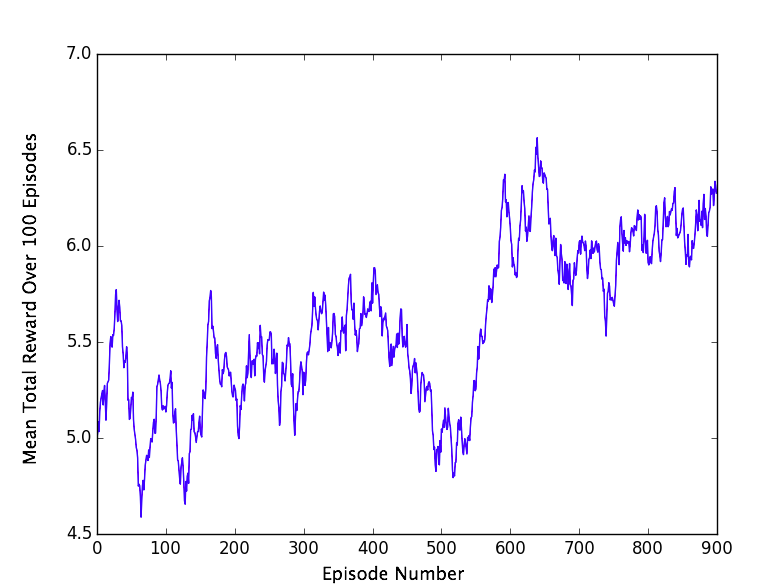
\includegraphics[scale=0.3]{progress_report.png}
\caption{Mario agent trained with a neural q-network with a hidden layer of 126 nodes. The agent was trained for 1000 episodes of the same level seed 3 and difficulty 1. The initial exploration factor was 1.0, and this decreased by 0.05 every 100 episodes, until stopping at 0.1. The total reward gained by the agent was summed over each episode, and the running average of 100 episodes is shown here.}
\end{center}
\end{figure}
  
 We have yet to optimize our agents over the space of configuration parameters (learning rate, regularization, max number of experiences, probability of remembering an experience, discount factor on future rewards). Also, we have not yet attempted to train an agent on a particular level, and evaluate its performance on a new level of a different difficulty level.
 
\section*{Acknowledgments} 
 
None.

\bibliography{final_report}
\bibliographystyle{icml2014}

\end{document} 


% This document was modified from the file originally made available by
% Pat Langley and Andrea Danyluk for ICML-2K. This version was
% created by Lise Getoor and Tobias Scheffer, it was slightly modified  
% from the 2010 version by Thorsten Joachims & Johannes Fuernkranz, 
% slightly modified from the 2009 version by Kiri Wagstaff and 
% Sam Roweis's 2008 version, which is slightly modified from 
% Prasad Tadepalli's 2007 version which is a lightly 
% changed version of the previous year's version by Andrew Moore, 
% which was in turn edited from those of Kristian Kersting and 
% Codrina Lauth. Alex Smola contributed to the algorithmic style files.  
